%\pagebreak

%\begingroup\thispagestyle{empty}

%\begin{tikzpicture}[remember picture,overlay]
%\node at (4.6,-8.5)
%  {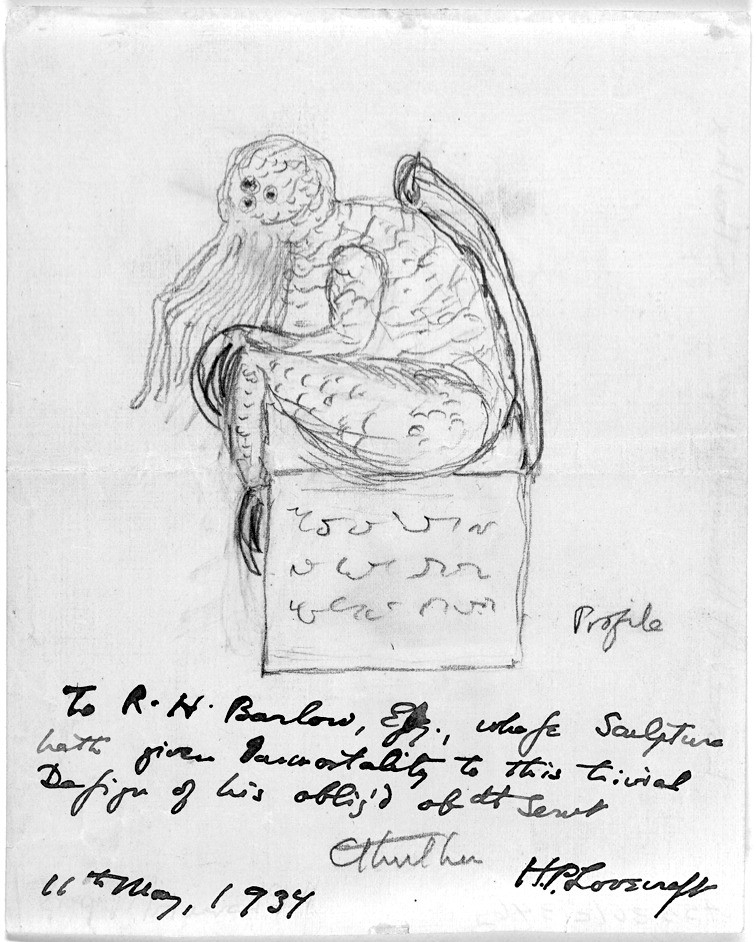
\includegraphics[width=\paperwidth]{img/cthulhu1.pdf}};
%\end{tikzpicture}

\clearpage
\thispagestyle{empty}
\AddToShipoutPicture*{%
  \AtPageCenter{%
    \makebox(0,0){%
      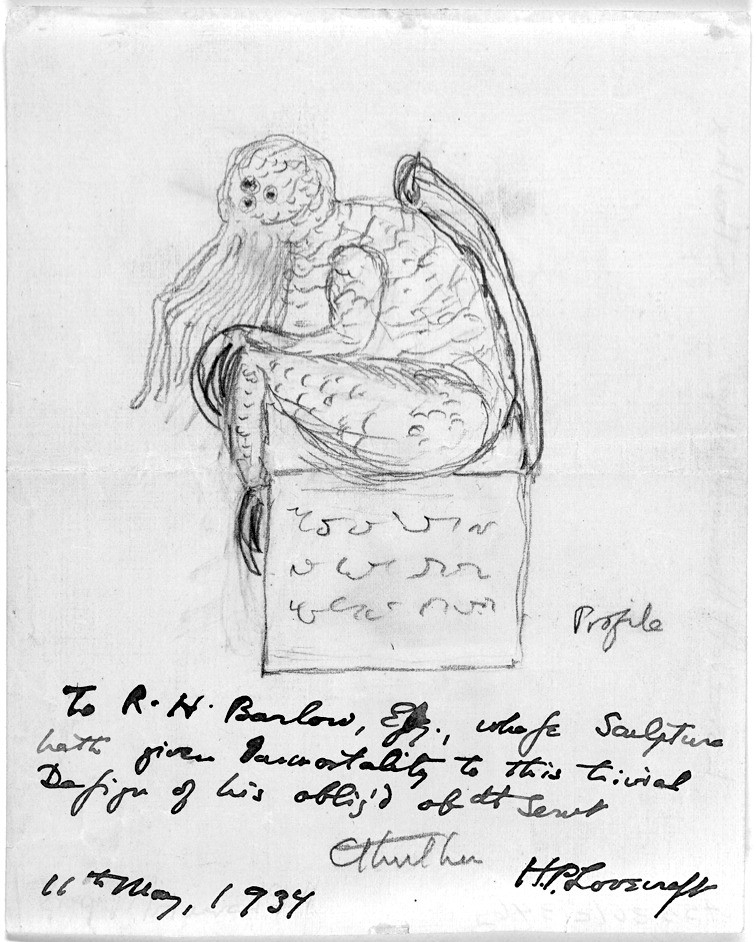
\includegraphics[width=\paperwidth,
                       height=\paperheight,
                       keepaspectratio]{img/cthulhu1.pdf}%
    }%
  }%
}
\null\clearpage % força a emissão da página e evita “vazar” para a próxima

%\pagebreak

\hyphenation{baseada}
\hyphenation{dread-ful}
\hyphenation{Moore}


\chapter[Introdução, \emph{por Dirceu Villa}]{Introdução\smallskip\subtitulo{De homens e 
monstros:\break Lovecraft e o horror}}
\markboth{Introdução}{}

\begin{flushright}
\textsc{dirceu villa}
\end{flushright}

%\section{Aberrações estadunidenses}

\noindent{}\textls[-15]{Howard Phillips Lovecraft já foi largamente traduzido e lido
no Brasil, e os fatos de sua vida são também bastante notórios: nascido
em Providence, Rhode Island, no topo dos \textsc{eua}, lugar quase enfiado nas
águas do Atlântico, Lovecraft veria seu pai morrer ainda cedo de
complicações da sífilis, que o enlouqueceram (dizia coisas bizarras ao
filho), e sua mãe, em consequência, teria passado o resto da vida em
amargura (paparicando Lovecraft e punindo-o psicologicamente
na mesma medida), o que fez com que o garoto ficasse muito próximo do
avô, Whipple Van Buren Phillips, rico empreendedor. Teve uma
infância com o mesmo aspecto de seus contos, obrigado a percorrer
quartos escuros, imaginando diabretes de Gustave Doré perseguindo-o com
tridentes pela casa, descobrindo o sexo com desgosto em livros de
anatomia e decidindo aos cinco anos, nietzschianamente, que Deus não
passava de um mito, após ouvir dizer o mesmo sobre o Papai
Noel.}\footnote{O que se pode ler no importante e interessantíssimo
  documento autobiográfico, o ensaio ``A confissão de um cético'' (1922),
  no qual Lovecraft afirma que pouco antes já se dizia devoto
  muçulmano e se dava o nome de Abdul Alhazred (por seu fascínio pelas
  \emph{Mil e uma noites}), mais tarde imortalizado como o poeta
  árabe insano de sua ficção.}

A infância --- que ao menos tivera o conforto da riqueza do avô ---
acabou também cedo, com a desgraça empresarial seguida da morte do velho
homem por infarto: Lovecraft, a mãe e uma tia solteira foram então
lançados à pobreza e a um tanto de desespero. Obviamente, sua vida
escolar sofreu com as agruras familiares, e Lovecraft percorreu a escola
de modo errático até que o trajeto fosse interrompido em definitivo por
um colapso nervoso no segundo grau; o mais próximo que chega de
prosseguir com alguma educação formal é um curso de química que faz por
correspondência. Essa história frustrada lhe deixou marcas profundas de
um desejo de se provar intelectualmente diferenciado, especial, o que se
nota mesmo em sua escrita de ficção, muitas vezes na forma de avaliação
da inteligência (ou falta de) de seus personagens.

Interessado em ciências e de imaginação vivíssima, também alimentada
pela biblioteca do avô (onde desde muito cedo leu livros robustos, como
as \emph{Metamorfoses} de Ovídio e \emph{A rima do velho marinheiro} de
Coleridge, entre outros) e por uma rotina de recitação de Shakespeare
com a mãe, Lovecraft era por assim dizer um \emph{nerd avant la lettre},
uma fina sensibilidade cultivada --- e estraçalhada --- no alto da
sociedade industrial e mecânica, entre horrores psicológicos, ciência,
timidez erótica, desajuste social e medo do mundo, suscetível a colapsos
nervosos e insone.

Lovecraft não parece ter sido um tipo agradável, aspecto biográfico que
partilha com aquele de quem --- não sem bons motivos --- se diz que
descende: Edgar Allan Poe. Mas a passagem de Poe para
Lovecraft explica-nos igualmente um pouco da história dos \textsc{eua}, o país de
ambos, e onde ambos viveram quase anônimos: se Poe era um alcoólatra
neurótico, Lovecraft foi um ultraconservador paranoico, repleto de
preconceitos enraizados e violentos. Penso que a \emph{doença} --- se
pudermos utilizar a palavra com alguma licença poética --- de Poe, como a
de Lovecraft, é a \emph{doença da percepção}. Os dois notaram um complexo
de horrores futuros, ainda sem forma, mas que perturbavam suas finas
percepções. Se Poe herdou as visões perturbadoras do alemão E.\,T.\,A.
Hoffmann,\footnote{Contos como ``Os autômatos'' e ``O homem da areia'' são duas das mais importantes
  peças desse gênero de literatura, cujos desdobramentos reais Sigmund
  Freud teria a felicidade de nomear \emph{Das Unheimliche} [O inquietante,
  1919], no valioso ensaio que define um tipo recente de horror, o do
  familiar-estranho, que veremos adiante.} Lovecraft herdaria, por sua
vez, as de Poe.\footnote{E há quem diga que Stephen King herdou de
  Lovecraft. O que não parece muito exato, porque o maciço e contínuo
  sucesso multimilionário torna King menos perceptivo. Como King mesmo
  disse, sua literatura é o equivalente de um Big Mac. Nada contra o Big
  Mac, nem contra King, mas isso explica por que o autor detestou a
  adaptação cinematográfica do seu \emph{O iluminado} (1977) por Stanley Kubrick naquela obra-prima de 1980: sua percepção,
  como artista, está limitada aos efeitos, não vê estrutura.}

Haveria outro ponto fundamental para entender a estrutura
mental do horror lovecraftiano: Mary Shelley, com seu
\emph{Frankenstein} (1818). Lá se encontra pela primeira vez o tipo de
horror científico que se entrevira nos autômatos de Hoffmann, ele mesmo
um passo adiante das narrativas que o grupo de Byron leu naquela famosa
estadia na Suíça, o \emph{Gespensterbuch} (O livro de fantasmas, 1811--1815)
de Johann August Apel e Friedrich Laun, em que seus organizadores reúnem
e reescrevem antigas narrativas folclóricas de horror germânico. Mary
Shelley leva essa narrativa a um ponto que não teria sido possível imaginar
antes, trazendo o foco a uma absoluta \emph{hybris} da razão.\footnote{Para
  notar como Mary Shelley antecipou questões profundas da humanidade,
  basta lembrar da frase de Robert Oppenheimer, um dos
  grandes físicos a desenvolver o Projeto Manhattan, o da bomba de
  hidrogênio, após a explosão das bombas de Hiroshima e Nagasaki: ``os
  cientistas conheceram o pecado''. Mary Shelley soube muito antes,
  como a arte em geral o sabe.}

\textls[-8]{O subtítulo a \emph{Frankenstein}, ``Prometeu moderno'', é precisamente
o ponto: a luz da ciência, como sabemos, projeta sombras largas, e
Shelley o nota, pois afirma que escreveria dos ``medos misteriosos da
nossa natureza'', mas também, e sobretudo, do que surgiu nas conversas
dos escritores reunidos sobre ``a natureza do princípio da vida'', em
particular de um experimento do dr.\,Erasmus Darwin, que lhe
deixou a hipótese}\looseness=-1\footnote{``Eles falaram [\emph{eles} são Byron,
  Shelley, Polidori] dos experimentos do dr.\,Darwin (não falo do que
  o doutor realmente fez ou disse que fez, mas, mais ajustado ao meu
  objetivo, o que então teria sido feito por ele), que preservou um
  pedaço de verme num vidro até que de alguma maneira extraordinária
  ele começou a se mexer com movimentos voluntários. Não é assim, afinal,
  que se daria vida. Talvez o cadáver tenha sido reanimado; galvanismo
  já dera exemplo de tais coisas: talvez as partes que compunham a
  criatura pudessem ser manufaturadas, recompostas, e dotadas de calor
  vital'' (\textsc{shelley}, Mary. Author's Introduction. In: 
  \emph{Frankenstein}: or The Modern Prometheus. Nova York: The Modern
  Library, 1993).} \textls[-10]{que o próprio Lovecraft depois revisitaria em
``Herbert West -- Reanimator'' (1921--1922).}

De resto, como sabemos ao menos desde a frase atribuída a Joseph Heller,
autor de \emph{Ardil-22} (1961), ``o fato de ser
paranoico não quer dizer que não estejam atrás de você''. O século~\textsc{xx}
geraria uma quantidade realmente espantosa de indivíduos visionários e
adoecidos, desconfiados da máquina gigantesca gerada por um Estado
crescentemente policial, guerras de dimensão nunca antes vista e a ação
viciante da propaganda midiática narcótica para as massas. Este século~\textsc{xxi} 
segue e aprofunda o costume, quando as teorias da conspiração (um
bom número delas já nem mais \emph{teorias}, mas \emph{fatos} de
conspiração) são a mais popular vertente dos horrores escondidos sob a
aparência cotidiana de normalidade. Diria que Lovecraft desempenha um
papel estrutural nisso, e eis porque, como veremos, ele é onipresente
hoje.\looseness=-1

\section{Um mundo estranho}

Os \textsc{eua} surgiriam no ano da independência de 1776, mesmo ano, aliás,
curiosamente, de surgimento da incompreensível sociedade secreta dos
Illuminati --- criada pelo advogado bávaro Adam Weishaupt ---, com 
a qual compartilham laços maçons, como vemos no símbolo maçônico da pirâmide 
com o olho que tudo vê, impresso no dólar, dinheiro estadunidense, símbolo do 
poder na
sociedade;\footnote{E nos
  lemas \emph{Annuit coeptis} [``Tem aprovado''] e \emph{Novus ordo
  seclorum} [``Nova ordem dos séculos''], em que a palavra ``ordem'' não
  deve passar despercebida. A maçonaria também desempenhou papel
  fundamental na Revolução Francesa, porque os pedreiros-livres tinham
  de ser ocultos, dado que o \emph{Ancien Régime} não via com bons olhos
  o sistema burguês-industrial crescente. E como escreve Walter Isaacson
  sobre um dos mais importantes agentes da independência estadunidense
  (e da Constituição do país), Benjamin Franklin: ``Franklin se tornou
  um maçom fiel. Em 1732 ajudou a esboçar o regimento interno da loja da
  Filadélfia, tornando-se Grão-Mestre dois anos mais tarde e imprimindo
  sua constituição'' (\textsc{isaacson}, Walter. \emph{Benjamin
  Franklin}: An American Life. Nova York: Simon \& Schuster, 2003, p.\,106).}
 mas precisamente um \emph{novo tipo} de poder, o que faz os
bastidores assumirem o centro de irradiação, uma vez que a democracia se
convenciona e passa a ser usada apenas como negociação com as massas,
com as decisões declaradamente se fazendo a portas fechadas, longe dos
olhos de quem poderia não compreender a frieza do que chamam estratégia,
ou de quem poderia se horrorizar com certos métodos decisórios.

Os \textsc{eua} do \textsc{xix} são portanto os \textsc{eua} do esforço de criar uma nação não
apenas autônoma, mas nova sob todos os aspectos, uma nação que
combinasse ciência (não em abstrato, mas como aplicação técnica),
um modelo de democracia,\footnote{\textls[-15]{Democracia já foi muitas coisas
  diferentes --- algumas bem pouco democráticas --- desde seu nascimento
  registrado, em Atenas. Algumas de suas versões aceitavam escravidão; a
  maior parte de seus modelos excluía as mulheres, por exemplo.}\looseness=-1} um
zelo pelo dinheiro segundo a ética protestante weberiana\footnote{A
  ética puritana, originada no calvinismo da predeterminação dos
  destinos e da moralidade individual, propõe uma vida de trabalho
  persistente e de circunspecta obediência aos deveres. Um dos deveres
  fundamentais é com o dinheiro, porque os deveres são todos do mundo
  temporal, como o é trabalhar. Não ter dívidas, ser de caráter aplicado
  e sistemático, profissional racional da divisão do trabalho e
  empenhado no lucro, visto não apenas como um bem da
  coletividade, mas também como um dever individual daquele a
  quem Deus aponta esse caminho, estabelecem a famosa definição do
  economista e jurista alemão Max Weber em sua obra
  fundamental \emph{A ética protestante e o espírito do capitalismo}
  (1904--1905).} \textls[-10]{e, sobretudo, essa estranha relação, de sombras, com o
poder. O ponto fundamental é que se foi criando uma sociedade --- desde
a divisão do conhecimento e do trabalho, o uso das máquinas da Revolução
Industrial,} a administração do crédito pessoal por bancos e a categoria
de administração da \emph{res publica} por políticos que se distanciam
de modo progressivo da esfera efetivamente pública das ações --- em que
o indivíduo é afastado dos meios da sua existência, e da existência
comum com os outros, por camadas e camadas que efetuam, sem que
ele saiba quais e para quê, suas decisões, uma variação moderna do
afastamento exercido pela antiga sociedade estamental.

As sombras são o ponto psicossocial dessa literatura de horror (até
freudiano, como se verá), pois há o poder publicamente proposto, e há o
poder de fato; se sempre foi assim,\footnote{Basta lembrarmos de
  uma das frases famosas de Elizabeth Tudor, a rainha
  Elizabeth \textsc{i}, %\emph{We princes, I tell you, are set on stages}, 
  ``Nós,
  príncipes, somos postos em palcos'', cristalizando a noção, de resto
  elementar, de que a política monta uma grande fanfarra publicamente e
  faz o sinal de Harpócrates para o que urde, aí de fato, nos
  bastidores.} amplifica-se cada vez mais a oposição entre
aparência pública e prática reservada, sobretudo porque é
na última que se decidem os rumos político-econômico-sociais e até mesmo
culturais. O curto-circuito não é percebido de modo geral pela população
--- que costuma obedecer à ordem vigente sem muito ruído ---, mas é
nesse escuríssimo armário de esqueletos da sociedade que vive a
imaginação daqueles dois estadunidenses, Poe e Lovecraft. Lovecraft em
particular: seu fascínio pelo distúrbio da consciência, pela ciência
ficcional frankensteiniana, pela interferência alienígena, pela agressão
simbólica sobre a psique e pela insegurança existencial generalizada são
pontos de intensa vibração de uma \emph{angst} que além de não ter
envelhecido está mais viva do que nunca.\looseness=-1

O cerne da literatura de Lovecraft está no fato de que desconfia,
que intui que as maiores forças deste mundo operam nas sombras:\footnote{Para
  citar de passagem um número de exemplos na obra de Lovecraft que o
  confirmam: os ratos estão dentro das paredes, as abominações
  pré-humanas vivem sob o oceano, a própria morte parece apenas um
  segredo ocultado que é preciso sacar da escuridão, a música inumana
  vem de um terrível diálogo com as sombras etc.} sua prática é notar o aberrante, mesmo exagerá-lo para efeito educativo (e que,
como deformação extrema, parte da alegoria e tende à caricatura). Quem
pensa que o faz pelo motivo trivial de tentar a ssustar seu público, ou
porque sua psicologia literária, como a de Poe, fosse imatura, se engana
--- sobre os dois. Não se trata de fantasia por irrealidade ou
imaturidade, mas de uma fina percepção adoentada por uma sociedade que
castiga essas percepções. Se ambos tivessem surgido na Grécia, por volta do
século~\textsc{v} a.C., é bem provável que tivessem escrito tragédias para o
apreço do professor Aristóteles, ou que, surgindo no meio do século~\textsc{xvi}
na Inglaterra, escrevessem peças macabras e sanguinolentas à espanhola,
como fez Thomas Kyd. Nascendo onde e quando nasceram, escreveram o que
se chama, sempre com algum desdém criticamente supercilioso,
literatura fantástica.


\section{Literatura fantástica: contra\break a definição desdenhosa}

``Fantástico'', em sua origem etimológica, é, nos diz Aristóteles,
\emph{phos}, ou ``luz'', em grego.\footnote{Sobre esse assunto em
  particular, ler o importante artigo de Jorge Sallum, ``Phantasía e
  retórica estoica'', publicado na revista digital \emph{Germina
  Literatura} em março de 2008.} As antigas teorias sobre
\emph{phantasía}\footnote{\textls[-5]{\textsc{garin}, Eugenio. \emph{Phantasia} e
  \emph{imaginatio} fra Ficino e Pomponazzi. In: \textsc{fattori},\,M.; 
  \textsc{bianchi}, M.\,L.
   (ed.). \emph{Phantasia-Imaginatio}, atti del \textsc{v} Colloquio Internazionale del
  Lessico Intellettuale Europeo (Roma, 9--11 jan. 1986). 
  Roma: Edizioni dell'Ateneo, 1988.}} vinham do
campo filosófico estoico que discutia as bases do que hoje chamamos, sem
filosofia alguma, realidade: em grego distinguia-se entre
\emph{phantásmata} (o que a mente encontra no mundo) e
\emph{phantastikón} (o que a mente concebe por si, sem a necessidade de
achar aquilo no mundo),\footnote{De modo que ``fantasma'' e
  ``fantástico'' têm origem etimológica comum, o que não é casual nem
  mesmo se se quiser pontuar tudo o que, depois, separou semanticamente
  as duas palavras.} duas palavras importantes para o propósito
filosófico e seríssimo de explicar realidade, imaginação e sonho. Hoje,
quando o máximo que se lê é pouco mais do que uma centena de dígitos,
filosofia obviamente não é possível; quando era, os estoicos surgiram
com uma sagacidade notável, propondo que deus, como \emph{logos}, está
em tudo, e, estando em tudo, essa fagulha criadora ativa no
\emph{phantastikón} uma concreção do campo imaginativo, uma condensação
das quase inapreensíveis \emph{lógoi spermatikói}, ou ideias seminais,
aquilo que, seguindo Platão, chamaríamos \emph{mundo das ideias}, e
que Carl Gustav Jung bem mais tarde apropriaria sob o nome de
\emph{inconsciente coletivo}.\looseness=-1\footnote{\textls[-15]{Há também uma conexão com a
  antropologia difusionista --- o conceito de \emph{Kulturkreise}, ou
  ``círculos de cultura'', de Leo Frobenius, no começo do século~\textsc{xx}.}\looseness=-1}

Fantástico, nesse sentido, serviu também, na Antiguidade, para a
circunscrição dos sonhos premonitórios na \emph{Onirocrítica} --- não
foi Sigmund Freud quem inventou a interpretação dos sonhos ---, como
definiu Artemidoro de Dáldis (século~\textsc{ii} d.C.): sonhos com a força de
intuir o futuro;\footnote{Ou, nas palavras de Artemidoro: ``ficção
  multiforme da alma que anuncia os bens e os males futuros''
  (\textsc{daldis}, Artemidoro de. \emph{El libro de la interpretación
  de los sueños}. Madri: Akal, 1999, p.\,70). Os sonhos premonitórios
  desempenham um papel particularmente interessante em \emph{O chamado de
    Cthulhu}, sobretudo se os virmos à luz da antiga onirocrítica.} ou
de rasgar uma delicada fenda dimensional, espaciotemporal, como
imaginaríamos depois da Relatividade de Einstein, e também com a parte
da ficção científica atual que escreve sobre o papel do Grande Colisor
de Hádrons, o gigantesco túnel para colisão atômica metido num buraco da
fronteira entre França e Suíça.

O poder de plasmar a realidade não foi aludido apenas pelos antigos ou
por descendentes do poderoso conhecimento oculto no Renascimento, como a
noção de \emph{disegno interno} faz ver na escultura italiana:\footnote{Como
  explica Federigo Zuccaro em seu tratado \emph{L'idea dei
  pittori, scultori ed architetti}, o \emph{disegno interno} (1607) é
  \emph{luce dell'intelletto}, e um \emph{oggetto immateriale}.
  Michelangelo Buonarroti, como outros, assinalava a
  preexistência da figura já na pedra, que ele apenas liberava.} para
todos aqueles que admiram a arte cinematográfica de David
Lynch,\footnote{Todos os filmes de David Lynch, como os de Stanley
  Kubrick, são códigos para mecanismos de imaginação e para a relação
  complexa entre os conceitos de mente, realidade e manipulação
  ritualística, pelo poder, das forças imaginárias.} foi exatamente o
que Lynch fez no oitavo episódio da terceira temporada de
\emph{Twin Peaks} (2017). Assistindo ao nascimento de uma nova categoria
de horror humano na explosão da primeira bomba atômica no Novo México,
em 1945, a Señorita Dido e o Bombeiro --- seres metafísicos em seu
não lugar metafísico que lembra um cinema --- geram a partir de intensa
luz uma esfera dourada, então lançada na direção da Terra por um
aparelho cujo funcionamento, aliás, não é diferente do da máquina de
metafísica amorosa inventada por Marcel Duchamp em seu \emph{Grand
Verre}, ou \emph{La mariée mise à nu par ses célibataires, même}
(1915--1923).

Apesar do desdém da crítica (que vem sendo revertido lentamente nos
últimos anos), o fantástico na literatura pode fazer recuar suas
nobilíssimas raízes até as fábulas gregas de Esopo,\footnote{Falo apenas
  das raízes ocidentais. Naturalmente, o Oriente está também repleto
  dessas raízes do fantástico.} que punham os animais a falar; aos
espetaculares feitos de transformação nas \emph{Metamorfoses} de Ovídio
(que Augusto de Campos já emparelhou à narrativa cinematográfica
muitíssimo \emph{avant la lettre}),\footnote{\textsc{campos}, Augusto de. Metamorfoses das
  metamorfoses. In: \emph{Verso reverso
  controverso}. São Paulo: Perspectiva, 1978, p.\,191.} depois emulados por
Dante na \emph{Comédia},\footnote{Em particular no Canto \textsc{xxv} do \emph{Inferno},
  quando Dante proclama sua vitória sobre as metamorfoses ovidianas por
  ter concebido a transformação de ladrões em répteis num processo que
  jamais se conclui em qualquer uma das duas formas cambiantes.} com
seus espantosos monstros teológicos descritos em requintes gráficos; ou
às muitas viagens à Lua, de Luciano de Samósata a Cyrano de Bérgerac (o
autor, não o personagem derivado dele por Rostand); mas penso que um
ponto de inflexão se encontra no poema de John Milton, \emph{Paraíso perdido} (1667).

Lá, no verso 13 do Livro \textsc{i}, Milton define seu longo poema como
\emph{adventurous song}, ou ``canção aventuresca''. Não é uma definição
casual e sem importância: imitando tanto a épica greco-latina como o
poema teológico de Dante, seu poema nasce confuso e sem gênero claro.
``Sem gênero'', até o século~\textsc{xviii}, significa uma anomalia em que as
onipresentes regras retóricas de composição patinam, e é nesse patinar
que o poema de Milton, não sendo épico nem teológico, se torna
aventuroso, ou fantástico.\footnote{Os ferimentos das armas comuns de
  anjo contra anjo numa batalha se fecham com a velocidade que
  aprendemos a ver em um dos heróis mutantes da Marvel Comics, o
  \emph{x-men} Wolverine. Daí que Deus presenteie Miguel com uma espada
  especial, para matar anjos, que rasga a pele de Lúcifer, para terror
  deste: \emph{Then Satan first knew pain} [``Então Satã enfim conheceu
  a dor'', Livro~\textsc{vi}, v.\,326], com a ferida aberta de onde manava um
  ``humor nectáreo'', fluido sanguíneo, que é, anota Milton com zelo
  etnográfico, o que ``espíritos celestiais'' devem sangrar.\looseness=-1}

O que era, em Homero ou Virgílio, ação demonstrável de virtudes civis,
claramente calcadas em aspectos mitológicos ordenados para essa
exemplaridade civilizacional, se torna ação aventuresca em Milton; o que
era teologia em Dante, estipulando uma \emph{ordo} (ordem) baseada no
conceito de \emph{rectitudo} (retidão), catolicamente definido, e onde o
mundo dito pagão se torna alegoria de perversidade antinatural (Cérbero,
o cão de três cabeças, fora da natureza; o Minotauro, aberração de duas
origens diversas; os Centauros, emenda de homem e cavalo) entendida como
a multiplicidade falsa e mortal contra a verdade eterna e imutável de
Deus, torna-se em Milton a disputa muito dúbia de Lúcifer com o próprio
Deus, na qual episódios como a entrada secreta da Serpente no Paraíso,
ou o combate que Lúcifer dá aos anjos com canhões de fabricação
infernal, nada têm da gravidade dos gêneros antigos, mas propõem pela
primeira vez o que se leria como ligeireza do registro fantasioso, que
não é efetivamente crível em nenhum nível de apreensão do
texto,\footnote{Isto é, depende daquela operação definida por Coleridge
  como a \emph{suspension of disbelief}, ou a ``suspensão da
  descrença''. Nas \emph{Lyrical Ballads} que compôs com Wordsworth, a
  parte de escrever sobre ``personagens sobrenaturais'' lhe havia
  cabido, mas não de qualquer jeito, ``de modo a transferir de nossa
  natureza íntima um interesse humano e uma semelhança de verdade
  suficiente para reclamar a essas sombras da imaginação aquela
  voluntária suspensão da descrença por um momento, que constitui a fé
  poética'' (\textsc{coleridge}, Samuel Taylor. Biographia Literaria. In:
  \emph{The Major Works}. Edição, introdução e notas de H.\,J.\,Jackson. Oxford: Oxford University
  Press, 2008, p.\,314).} autonomizando a imaginação do irreal dentro de
uma aventura jamais dita em prosa ou rima.\looseness=-1

Como se percebe pela minha última frase acima, isso já havia ocorrido
antes de Milton --- e terá influído em sua própria escrita --- no
\emph{Orlando furioso} de Ludovico Ariosto, poema em que
pessoas voam nas costas de um grifo, em que as espadas de heróis matam
magicamente centenas de inimigos etc. Ariosto dá sentido ao conceito
posterior de \emph{fantasia}, como de \emph{aventura fantástica}, e que
antes já compareciam mesmo na invocação do poema de farsa épica, o
\emph{Baldo} (1517) de Teofilo Folengo: \emph{Phantasia mihi
plus quam phantastica venit} [\ldots{}] \emph{cantare}, ou ``Minha fantasia, bem
mais que fantástica, vem [\ldots{}] cantar'', no estilo que ficou conhecido,
já da proposição mesma de Folengo, como macarrônico, no molho
espesso de latim e italiano misturados.

A própria proposta de Ariosto era contar os feitos de fúria de
Orlando --- ``fúria'', ali, entendida como em sua raiz latina,
\emph{furor}, ``loucura''. As ligações da loucura com o
sonho (e a poesia) são as que lemos em todo o passado da arte
ocidental: estão por exemplo nos autos do processo inquisitorial contra
o pintor Paolo Veronese, que se defendeu da acusação de
heresia pronunciando sua inocência por fazer entender à Inquisição
veneziana que ``nós, pintores, utilizamos a mesma licença que poetas e
loucos''; estão, também, em \emph{Midsummer Night's Dream} (Sonho de uma
noite de verão, 1596), peça de sonho de William Shakespeare,
e em lugares filosóficos da literatura numerosos demais para listar
aqui, e todos ainda sem demarcação de limite estilístico, que viria
depois.\looseness=-1

\textls[-5]{Por isso é importante relembrar ao menos o poema da ``Rima do velho
marinheiro'', de Samuel Taylor Coleridge, que Lovecraft leu
ainda criança: um conviva numa festa de casamento é abordado pelo velho
marinheiro do título, homem condenado a narrar para sempre o infortúnio
seu e de sua equipagem, porque durante a viagem ele transgrediu o tabu
de matar um albatroz, desencadeando, assim, a maldição sobrenatural dos
mares sobre seu navio.}

As visões daqueles seres flutuantes e angélicos, a tripulação morta-viva
e fantasma que se ergue para completar a viagem fatal, os brilhos na
escura água do oceano e os encantos do horror, além da música mágica dos
versos, têm muito da nova exploração de campos imaginativos, e uma fonte
erudita: as discussões antigas para a delimitação entre \emph{phantasía}
e \emph{imaginatio}, fundamentais para aqueles que por exemplo viveram o
que chamamos Renascimento, pois, platônicos como eram, aquelas
duas coisas precisavam ser compreendidas e controladas para produzir
efeitos saudáveis, pois entendiam, com seu mestre grego, o \emph{terror
sagrado} da imaginação, que afetava a realidade de modo direto; quero
dizer, como acima o disse, o efeito de \emph{plasmar} a realidade (a
velha teoria estóica do \emph{pneuma}). Tinham receio: queriam conhecer
para usar com propriedade esse poder.

Não tinham esse receio os homens do fim do \textsc{xviii} e de todo o \textsc{xix} (a
partir do \textsc{xx} ninguém mais se preocupa com o assunto, e quer apenas
dominar seu público com uma imaginação poderosa que o submeta): para
eles havia chegado a hora de abrir essa caixa de Pandora, porque toda
``superstição'' havia sido vencida no século das Luzes. Os chamados
subgêneros de ficção científica, horror,  fantasia
medieval, e mesmo a literatura policial são produtos de meados
do século~\textsc{xix} e começo do~\textsc{xx}:\footnote{Alguns dos nomes de pioneiros
  fundamentais nesses subgêneros (alguns, contemporâneos de Lovecraft):
  Jules Verne, Arthur Conan Doyle, H.\,G.\,Wells, Agatha Christie.} nesses casos, o subgênero
passa a criar um grupo de leitores de gosto específico, interessado
naquelas narrativas imaginativas em parte como mero escapismo do
dia a dia massacrante do capitalismo industrial, em parte como
estímulo perceptivo-intelectual, e nesse caso há mesmo a
designação de ficção especulativa para a fantasia, o novo lar da
composição alegórica após a crise da retórica antiga como produtora de
práticas letradas.

A alegoria serve à ficção científica para propor futuros
avançados que espelhem a sombra do presente, e situar uma
hipótese extrema como crítica dos modos de vida, condicionados já desde
a Revolução Industrial por uma técnica desumanizada;\footnote{Basta
  citar alguns nomes e livros para constatar os mecanismos: Ray
  Bradbury, com \emph{Fahrenheit 451}; Arthur C.\,Clarke, 
  com \emph{2001: uma odisseia no espaço}, em colaboração com Stanley 
  Kubrick; Philip K.\,Dick,
  com \emph{Androides sonham com ovelhas elétricas?}, romance no qual se 
  baseou o filme \emph{Blade Runner}, de Ridley Scott, em 1982; entre outros,
  que também se desmembra na chamada ficção distópica, como
  achamos em \emph{Admirável mundo novo}, de Aldous Huxley; \emph{1984}, de
  George Orwell; \emph{A curva do sonho}, de Ursula K.\,Le Guin; e
  \emph{O conto da aia}, de Margaret Atwood; entre muitos outros e
  outras.} serve ao horror para hiperdimensionar com exemplaridade os
disparates da vida social, para trazer ao palco a camada escura e
escondida das pulsões humanas; serve à literatura policial para mostrar
que a leitura do mundo, nos predicados do que é a vida, só pode ser feita
aplicando-lhe argúcia e malícia; e serviu à fantasia dita
medieval para reconstituir a narrativa civilizacional da épica,
só que agora também com as tintas emprestadas do romance de formação, o
\emph{Bildungsroman}, no qual um ou mais personagens enfrentam a jornada
de transformação na vida, em geral de uma doce alienação juvenil para o
peso do conhecimento do mundo na maturidade, como se vê particularmente
na jornada de Frodo em \emph{O senhor dos anéis} (1954--1955), de J.\,R.\,R.\,Tolkien.\looseness=-1\footnote{É o que se pode ver também mais
  recentemente na série ainda incompleta de livros \emph{As crônicas de gelo e fogo} (1996--), de George R.\,R.\,Martin, que logo se tornou
  a série televisiva \emph{Game of Thrones}. A aproximação permanece
  válida mesmo que guardadas as diferenças grandes entre os
  empreendimentos de escrita de Tolkien e Martin. No caso de Tolkien, a
  experiência na guerra também constitui um forte condicionamento para a
  narrativa.}

Mas o tipo de fantasia de Lovecraft, ainda que se instale de modo mais
genérico dentro do horror, trouxe para o horror desenvolvimentos
inesperados, que depois influíram em toda a cultura de massas\footnote{Já
  expus acima parte dessa maciça influência, mas podemos pensar também
  em um filme como \emph{Alien} (1979), de Ridley Scott, e, no cinema,
  seria ainda necessário destacar o diretor mexicano Guillermo del Toro, uma vez que é provável não haver maior entusiasta de Lovecraft
  entre vencedores do Oscar; há John Carpenter, especialmente por
  sua refilmagem de \emph{The Thing} [O enigma de outro mundo, 1982] com as deformidades de seu
  transmorfo alienígena, e há também, entre muitos outros, Clive Barker, em sua obra escrita e cinematográfica, incluindo a parte de
  sua obra escrita em um domínio com larga influência lovecraftiana, as
  \textsc{hq}s; por fim, a chamada cultura nerd em peso lhe é devota, uma
  cultura que há poucos anos chegou ao \emph{mainstream} da indústria
  cultural.} e se traduzem numa confluência entre horror, ficção
científica e uma exploração psicanalítica das perturbações da percepção.
E Lovecraft era bastante consciente da divisão qualitativa naquilo que
se pode chamar literatura fantástica: em carta de 1934 a um Mr.\,Nelson, Lovecraft --- que estava já na última fase de sua escrita (viria
a morrer em 1937) --- assinala que uma coisa é Edgar Allan Poe, Ambrose
Bierce e Lord Dunsany etc., autores do que
chama ``autoexpressão'', e outra aquilo que define como algo ``composto
artificialmente para atender a certas demandas do leitor superficial \&
convencional''; para minha surpresa, ressalta que pouco do que fez lhe
satisfazia, e um desses poucos é o conto ``The Colour Out of Space'' [A
cor que caiu do espaço, 1927]: a tal cor, inexistente no nosso mundo,
chega à Terra em um meteorito.

Nesse conto, Lovecraft cria um dos conceitos mais complexos que a
literatura fantástica pôde desenvolver: se o mundo sofresse a
interferência de algo externo à experiência, essa intervenção, mesmo que
imotivada, produziria um efeito estrutural em quem a presenciasse, e de
modo irreconciliável com os demais, desencadeando atritos que cresceriam
até o conflito aberto. Fisicamente, a \emph{razão isotópica} de um
meteorito, uma pedra que vem do espaço, é diferente da de uma pedra
achada na Terra, protegida dos \emph{raios cósmicos}, ou da
\emph{radiação cósmica}, e por isso há entre elas uma diferença
fundamental, ainda que os elementos de constituição se achem na tabela
periódica: Lovecraft expande o dado científico em uma invenção
hipotética dos limites da civilidade, dos limites da percepção. Pode-se
até mesmo especular que a famosíssima série iniciada na \textsc{tv} por Rod
Serling nos anos~1950, \emph{Twilight Zone} --- que no Brasil ficou
conhecida como \emph{Além da imaginação} ---, terá partido de
ficções anteriores como essa de Lovecraft em específico.

É um experimento intelectual, e por isso o termo ``ficção
especulativa'' é tão apropriado para o melhor do que se escreve em
fantasia: está uns tantos passos adiante do que se chamou, com Émile
Zola no século~\textsc{xix}, romance de tese. O mesmo se dá em \emph{O chamado
de Cthulhu}, se lemos um dos trechos com especial atenção: quando os marinheiros estão na estranha ilha ciclópica e presenciam as
impossibilidades da geometria ``não euclidiana'' das construções.
Lovecraft descreve uma notável invenção ficcional do que depois, com a
física, poderíamos denominar \emph{anomalia de escala}, proposta no
conto como as regras clássicas do conceito de realidade em nível humano
sendo distorcidas quando se encontram coisas de fora desse espectro,
formas nas quais um ângulo supostamente reto pode se ``comportar'' como
obtuso.

A fantasia, como gênero de arte e literatura, se apropria de aspectos
dessa lenta sedimentação para amplificar os efeitos de uma visão
particular. A fantasia tem, em sua origem, como vimos, o mesmo ponto de
partida das antigas alegorias, porque ambas estabelecem um domínio
paralelo ao que está sendo dito, no sentido de que o que se diz é apenas
a instância inicial do que se projeta \emph{a partir} do texto. Mas a
despeito de suas enormes ambições, os subgêneros fantásticos já eram
rejeitados \emph{per se}, como vimos, estabelecendo-se antes em
publicações comerciais modestíssimas e esnobadas tanto pela crítica como
pelo ``bom gosto'' do respeitável público.\footnote{A efemeridade da
  coisa colaborava para o conjunto de preconceitos: não eram feitas para
  durar, impressas em papel vagabundo e para o consumo incauto das
  massas. Ao menos desde Charles Baudelaire, o maligno poeta
  de \emph{As flores do mal} (1857), o jornalismo, publicado em folhas volantes,
  era visto como algo passageiro, sem a importância de uma arte da
  duração, e espelho dos novos tempos afobados e rudes. Conquanto isso
  em parte seja verdade, deve-se lembrar que muito daquilo que foi e é
  feito para durar não passa de má arte e má literatura: em todos os
  veículos a maioria nunca presta, mas em todos os veículos, não importa
  como nem por quê, haverá sempre um núcleo de verdadeira qualidade
  diferencial.}

\section{Pulp Fiction: Weird Tales}

O nome \emph{pulp fiction} foi alçado ao patamar das expressões
cultuadas como se traduzisse um tipo de atmosfera, ou um tipo de
atitude, como também seus antecedentes britânicos dos \emph{penny
dreadfuls}.\footnote{Não por acaso, \emph{Penny Dreadful} recentemente
  foi o nome de uma série baseada naquele tipo de narrativa seriada em
  papel barato do fim do século~\textsc{xix} na Inglaterra, e reunia personagens
  originalmente desconexos, como os de \emph{Drácula}, o 
  dr.\,Frankenstein e sua criatura, dr.\,Jekyll, Dorian Gray, um lobisomem
  etc. Obviamente, o seriado veio depois das séries de \textsc{hq}s escritas por
  Alan Moore, com arte de Kevin O'Neill, \emph{A liga extraordinária}, iniciada em 1999, e
  que se utilizava precisamente da curiosa reunião de personagens
  famosos da literatura fantástica da Era Vitoriana na Inglaterra, já
  dentro do subgênero \emph{steampunk}.\looseness=-1} O \emph{pulp} vinha igualmente
do esforço de reduzir o custo de produção das edições, empregando a
polpa da árvore no fazer dela papel barato para as revistas de consumo
popular. Essas publicações, nos \textsc{eua}, começaram no fim do século~\textsc{xix}
e atingiram o pico de popularidade entre os anos 1920 e 1930, com
títulos como \emph{Argosy}, \emph{Spicy Mystery}, \emph{Marvel Tales},
\emph{Blue Book}, \emph{Horror Stories} e outros. Essas publicações,
homenageadas e levadas ao centro das atenções ao menos desde \emph{Pulp
Fiction} (1992), o filme de Quentin Tarantino, eram essas edições
ordinárias em brochura, com capas chamativas ou escandalosas, vendidas
por centavos em banca de rua, com textos que contavam histórias
misteriosas, eróticas ou horripilantes: às vezes, as três coisas juntas.\looseness=-1

Parte da nascente indústria de entretenimento estadunidense,
essas edições condicionavam o estilo dos autores a buscar de qualquer forma a atenção
pública (em geral de modo aberrante ou escandaloso para os padrões da
época), porque o sistema dependia necessariamente da popularidade dos
títulos, e então a crítica da época ignorava tais brochuras,
desprezadas como má literatura apelativa; parte dessa crítica não se
dedicava sequer a tentar entender o fenômeno, mas buscava impor uma
visão artística imóvel em seus cânones, moralista e carola sobre os
escândalos escritos --- como, mais tarde, aconteceria com as próprias
\textsc{hq}s sob a censura do macarthismo e do \emph{Comics Code} (de meados da
década de 1940 e 1950), que higienizaria as publicações de suas
inventadas imoralidades.

\textls[-7]{\emph{Weird Tales} (1922--1954, com algumas tentativas de retorno aqui e
ali) foi a publicação \emph{pulp} na qual Lovecraft publicou parte
considerável de seus contos, e onde começou sua notória série de
Cthulhu, com a história que leremos nesta edição; lá também foi onde
Robert\,E.\,Howard, seu amigo, começou a publicar \emph{Conan, o bárbaro},
as aventuras do bruto cimeriano hoje famosíssimo pelas \textsc{hq}s da Marvel
Comics e pelos (quem diria?) já velhos filmes com o então monossilábico
Arnold Schwarzenegger no papel principal. A revista, por seu acidentado
histórico de publicação, não obstante pôde contar com aqueles e outros
nomes notáveis, já na época entre seus pares, e universalmente em
retrospecto. Eram escritores que herdavam uma tradição antiga, como
vimos, mas também recente de uma nova cristalização de subgêneros, e que
ainda não tinham lugar de visibilidade, em parte porque fruto da
indústria de entretenimento, em parte porque exploravam, pioneiros,
novos aspectos da arte da escrita conforme aqueles âmbitos.}

Lovecraft era um dos poucos que, ainda que condicionasse em parte seu
estilo àquelas necessidades do tipo de publicação, não precisava
sequer tentar se acomodar ao público: sua imaginação era tão obsessiva e tão
múltipla que suas histórias se sobressaíam mesmo entre as mais
estranhas; sua escrita, orgulhosa e sentenciosa, repleta de
subentendidos e sombrias maquinações inumanas, de estilo hiperbólico,
repetitivo e grandíloquo, iria se tornar não apenas imediatamente
atraente como depois seria o padrão para muitos que o seguiram em
explorar aberrações perceptivas, o estranho-familiar ou criaturas
multidimensionais perturbando a existência aparente deste mundo.

\section{A linguagem para o horror}

A linguagem que lemos neste \emph{O chamado de Cthulhu}, mas também em toda
a obra de Lovecraft, é rigorosamente característica de seu autor; a
respeito disso, não obstante, resta observar que, dada a gigantesca
influência que surtiu não apenas em seu gênero de escrita, mas em
inúmeras manifestações da indústria de entretenimento, é assim um estilo
incorporado a uma variedade de outras coisas que, na aparência, sequer
teriam a ver uma com a outra. A influência de sua linguagem é maciça, e
esse é ainda outro motivo para considerá-la em específico por um
momento.\looseness=-1

Lovecraft é por vezes chamado erudito: ele não é. Seu
conhecimento é errático e para nas informações essenciais (ou mesmo nas
ideias preconcebidas) em vários aspectos.\footnote{O vodu, por exemplo,
  utilizado no conto de Cthulhu, vem da impressão muitíssimo
  superficial, caricata, ideológica e preconceituosa que a ocupação dos
  \textsc{eua} no Haiti (de 1915 a 1934) trouxe ao público. Um livro em
  particular, ligeiramente posterior ao conto de Cthulhu, \emph{A ilha da magia} (1929), do jornalista, explorador e ocultista William
  Seabrook, popularizou uma noção de zumbi nos \textsc{eua}
  (esse que mais tarde se tornaria a criatura morta-viva e canibal de
  George Romero e o monstro mais popular do horror recente) e as noções
  extremas das práticas vodu haitianas, uma vez que Seabrook narra seu
  livro a partir de uma sensacionalista experiência pessoal. Filmes como
  \emph{Zumbi branco} (1932), de Victor Halperin, foram baseados no
  livro de Seabrook.\looseness=-1} Há em sua escrita um uso abusivo de adjetivos e
advérbios com a tentativa de hiperbolizar ou intensificar a descrição;
por vezes, esses usos montam um sobre o outro, entupindo o texto. Não se
trata de um autor lutando para dizer o indizível, como se poderia
pensar, porque mesmo onde não está em jogo o indizível seu estilo é
redundante, sentencioso, repleto de advérbios sonoramente semelhantes e
de dupla adjetivação frequente:\footnote{Encontra-se esse tipo de escrita
  adjetival e hiperbólica em numerosos exemplos. Ofereço um da minha
  tradução: ``Fúria animal e licenciosidade orgíaca aqui se misturavam,
  em alturas demoníacas, com êxtases de uivos e guinchados que irrompiam
  e reverberavam pelos bosques noturnos como tempestades pestilentes,
  vindas dos abismos do inferno''; sequências de advérbios se acumulam
  em menos de uma página, como \emph{hurriedly}, \emph{curiously},
  \emph{virtually}, \emph{really}, \emph{especially}, \emph{deeply},
  \emph{apparently}, \emph{wholly}, todos tomados do meio para o fim da
  página 183 da edição dos \emph{Tales}, da Library of America (2005),
  em posições por vezes tão próximas que fazem eco um ao outro. Há
  muitos mais no texto completo, e deixo à discrição da leitora e do
  leitor percebê-lo.} por não encontrar o recurso exato, Lovecraft
acumula, tentando dobrar a percepção dos leitores com a hipérbole.

Busca um tipo de grandiloquência de tipo grave, na qual por vezes
derrapa, mas seu talento inequívoco de linguagem se mostra em muitos
lugares: por exemplo, sempre que relata aspectos científicos, ou com
linguagem de demarcação específica em seu uso, que é quando Lovecraft se
torna minucioso e objetivo (quase maquinal) na anotação do jargão
utilizado, seja em manchetes de jornal, relatos de sociedades
antropológicas, registros de equipagem de navio ou linguagem de boletim
policial.

Pedante, fascina por em parte instituir esse tipo de linguagem que se
juntaria ao patrimônio vocabular da narrativa gótica e de ficção
científica, e, em parte, por aderir aos estilemas mais exagerados,
superficiais e abundantes do gênero do horror, que em muitos aspectos
repetem e muitas vezes diluem procedimentos acháveis em Mary Shelley,
Edgar Allan Poe e Bram Stoker. Devemos também lembrar que a educação de
Lovecraft foi até meados do segundo grau (alega ter ido à Universidade
Brown, mas não se formou), e isso parece ter sido sentido como uma
mácula e uma vergonha, compensadas por um grande orgulho de seu
intelecto, demonstrado ostensivamente em sua escrita ficcional.

Seu intelecto era claramente amplo, sua curiosidade, onívora, mas as
lacunas de uma formação incompleta que cedeu, em algum ponto, ao mero
exercício repetitivo do gosto lhe deixou vícios notáveis de estilo, além de
ideias fixas. São esses vícios e essas ideias fixas, no entanto, que o
fizeram notório como escritor e o particularizaram em uma vasta
quantidade de praticantes dos gêneros populares da escrita fantástica de
seu período. Assim como o antecessor e modelo Poe, o orgulho, os medos,
as frustrações e os ódios foram um combustível inventivo a Lovecraft e lhe deram
nervura estilística particular, especialmente para criar monstros
inesquecíveis, como o deste conto.

\section{O Grande Cthulhu}

Cthulhu é a fantasmagoria mais popular do muito popular
Lovecraft, e o centro de sua série sobre os Grandes Antigos, as
gigantescas e incompreensíveis criaturas anteriores a esta Terra, tal
como ela é conhecida; alguns chamarão ``criação de um mito'', ou de 
``mitologia'', mas é sobretudo impreciso e hiperbólico dizê-lo: um mito
não se cria, um mito eclode no tecido da realidade por processos
sedimentares em uma cultura e toma séculos de desenvolvimento
coletivo e anônimo, como leitura daquela mesma realidade.\looseness=-1\footnote{Joseph
  Campbell, especialista em mitologia, diria, por exemplo, no início de
  sua entrevista sobre o tópico do mito com Bill Moyers: ``Esses pedaços
  de informação dos tempos antigos, que têm a ver com temas que basearam
  a vida humana, construíram civilizações e deram forma a religiões por
  milênios, têm a ver com problemas interiores, mistérios interiores,
  umbrais internos de passagem [\ldots{}]'' (\textsc{campbell}, Joseph [com Bill
  Moyers]. \emph{The Power of Myth}. Nova York: Anchor Books, 1991, p.\,2).}

Os Grandes Antigos derivam dos compêndios ancestrais de demonologia e de
grimórios, nos quais frequentemente se anotam informações detalhadíssimas
sobre aquelas criaturas, como se se tratasse de registro legal em
cartório: características físicas, manifestações propícias, elementos
associados, nomes, ação, sinais identificáveis e até mesmo assinaturas.
O mais famoso --- e penso mesmo que até mais acessível de todos esses,
por não codificar nenhuma doutrina --- é o \emph{Dictionnaire Infernal}
(primeira edição em 1818), de Jacques Albin Simon Collin de Plancy, ocultista francês.

Compêndio montado com substanciosos verbetes de gosto antropológico na
escrita, o \emph{Dictionnaire Infernal} de Plancy reúne um repertório
enorme de criaturas em diversas culturas (\emph{répertoire universel},
diz o subtítulo), com ilustrações que são quase icônicas na imaginação
coletiva, de tanto que foram reproduzidas. A galeria dos Grandes Antigos
claramente se inspira naquela meticulosa coleção, também pela forma
proposta aos demônios na Antiguidade, que --- como disse acima ao
mencionar Dante e suas aberrações infernais --- os constituía pela
mistura antinatural de formas e espécies.

A invenção de Cthulhu é algo central, e não apenas para Lovecraft: de
suas criaturas e ambientes de sonho --- ou melhor, talvez, pesadelo
--- é a mais famosa, e figura com o próprio Lovecraft em inúmeras
imagens de divulgação, como sua marca registrada. Vazou para a cultura
pop, e há desde estatuetas fidedignas à descrição no conto até
pequeninos e doces bichos de pelúcia estampados com seu nome. Alguns até
ouviriam mentalmente, de imediato, as memoráveis primeiras notas de
``The Call of Ktulu'', do álbum \emph{Ride the Lightning} (1984), do
Metallica, ao escutar o nome da criatura.\footnote{Dentre os estilos
  musicais, o metal é obviamente o meio mais lovecraftiano. O Iron
  Maiden, por exemplo, estampou os célebres versos do árabe insano de
  Lovecraft na pedra tumular de sua mascote, Eddie, na capa do álbum
  gravado ao vivo, \emph{Live After Death} (1985).}

E a criatura foi um modo para Lovecraft cristalizar numa imagem um tipo
específico de terror, que em geral se chama ``cósmico'', mas um cósmico,
penso, muito íntimo e literário; do literário veremos agora, do íntimo,
adiante. Em Cthulhu estão infusas as influências monstruosas daqueles
compêndios e grimórios, mas também um poema em particular. Se já havia
assinalado que o poema de Coleridge era base imaginativa para Lovecraft
de modo geral, um outro de Lord Tennyson em particular lhe
deu um bom tanto de linguagem grandíloqua e de atmosfera, isso sem falar de
aspectos da própria criatura.\footnote{Quem propôs a relação foi o
  Reverendo Robert\,M.\,Price, em seu livro \emph{H.\,P.\,Lovecraft and the
  Cthulhu Mythos}, de 1990.} O poema é ``O Kraken'', que traduzo
abaixo:

\begin{verse}\noindent
Sob os trovões nas altas profundezas,\\
Fundo no profundo abismo do mar,\\
Sem sonho, o sono antigo sem surpresa\\
Dorme o Kraken: a tênue luz solar\\
Dança em seu corpo sombrio, e acima\\
Flutuam esponjas grandes, milenares;\\
Ao longe, a luz doentia anima\\
Polvos gigantescos, que aos milhares\\
Saem de incríveis grutas e cavernas\\
Com longos braços no verde dormente,\\
Que lá esteve e estará por eras;\\
No sono, vermes do mar são sua presa\\
Até que o fogo aqueça as profundezas;\\
E homens e anjos verão, finalmente,\\
Erguida num urro de morte, a fera.\footnote{``\textsc{the kraken}//\,Below the
  thunders of the upper deep;/\,Far, far beneath in the abysmal sea,/\,His
  ancient, dreamless, uninvaded sleep/\,The Kraken sleepeth: faintest
  sunlights flee/\,About his shadowy sides: above him swell/\,Huge sponges
  of millennial growth and height;/\,And far away into the sickly
  light,/\,From many a wondrous grot and secret cell/\,Unnumber'd and
  enormous polypi/\,Winnow with giant arms the slumbering green./\,There
  hath he lain for ages, and will lie/\,Battening upon huge sea worms in
  his sleep,/\,Until the latter fire shall heat the deep;/\,Then once by man
  and angels to be seen,/\,In roaring he shall rise and on the surface
  die'' (\textsc{hodder}, Karen [org.].\emph{The Works of Alfred Lord Tennyson}. 
  Ware: Wordsworth, 2008, p.\,46).}
\end{verse}

Nele estão as vertiginosas direções das ``altas profundezas'', o monstro
que dorme no fundo do mar, o verdor de sua pele, os efeitos da
tempestade, a adjetivação que diz ``doentia'', ``sombrio'', as dimensões
inqualificáveis do corpo descomunal e, naturalmente, o próprio Kraken:
monstro marinho e cefalópode da mitologia escandinava, o polvo gigante
que assombrava as antigas sagas em verso se metamorfoseou algum tanto no
cefalópode antropóide Cthulhu. Lovecraft pôde encontrar, naquele monstro
antigo que remontava, um código de seus próprios horrores, mas que
funcionou especificamente porque o verdadeiro mergulho no medo de um é o
mergulho no medo de todos.

\emph{Watchmen} (1986--1987), a \emph{graphic novel} de Alan Moore e Dave
Gibbons, utilizou um efeito lovecraftiano que sublinha o que dizia
anteriormente sobre a força da fantasia, da concreção do campo
imaginativo e dos códigos dos nossos medos. A dada altura, um monstro
viscoso e tentacular se manifesta destruindo parte de Nova York. O
monstro havia sido o resultado de uma \emph{engenharia}, cuja peça
fundamental fora o cérebro clonado de um humano sensitivo: 

\begin{quote}
O sensitivo
era a chave [\ldots{}] o cérebro era uma caixa de ressonância psíquica [\ldots{}]
Codificamos muitas informações naquele sinal. Informações terríveis. As
descrições de Max Shea de um mundo alienígena, as imagens de Hira Manish
e os sons de Linette Paley\ldots{} Além dos que morreram imediatamente pelo
choque, muitos ficaram loucos pelo súbito dilúvio de sensações
grotescas.\footnote{\textsc{moore}, Alan; \textsc{gibbons}, Dave. \emph{Watchmen}.
  Burbank: \textsc{dc} Comics, 2014, p.\,391--392. [1ª ed. 1986].}
\end{quote}

O texto de Moore sobre o impacto da criatura explodindo sobre a cidade
mostra que a arma alienígena fora composta pela informação extraída de
artistas da palavra, das imagens e dos sons,
amplificados por uma mente sensitiva; precisamente, aliás, como
Lovecraft já propunha, seja em \emph{O chamado de Cthulhu} com o jovem
escultor Wilcox, seja em ``A música de Erich Zann'' com a música do
próprio Zann, e, diríamos, com as palavras de Lovecraft \emph{lui-même}.
Moore, inventando sua criatura cthulhiana, fornece aos leitores atentos
uma definição do complexo imaginativo que os escritores põem a andar
como criaturas entre nós, devolvendo de maneira sintética as impressões
coletivas que recebem do mundo. E é aqui que achamos a oportunidade de
ir às impressões íntimas de Lovecraft, codificadas em sua ficção.

\section{Um mundo invertido}

\emph{My world is Providence}, afirmou Lovecraft. E poderíamos dizer,
talvez com mais propriedade do que ele disse de si, que seu mundo era
sobretudo sua mãe. Se de Providence imaginou a vizinha Arkham\footnote{O
  Asilo Arkham, famoso por reunir os criminosos insanos da corte de
  vilões de Batman, da \textsc{dc} Comics, vem diretamente de Lovecraft, que o
  inventou em ``The Thing on the Doorstep'' (A coisa na soleira da porta, 1933, publicado em
  \emph{Weird Tales} em 1937): ``É verdade que pus seis balas na cabeça
  de meu melhor amigo, mas espero ainda demonstrar com este relato que
  não sou um assassino. De início serei chamado insano --- mais insano
  do que o homem contra quem disparei em sua cela no Sanatório Arkham'' [tradução minha]
  (\textsc{lovecraft}, H.\,P. \emph{Tales}. Nova
  York: The Library of America, 2005, p.\,692).} ---
cidade de que até mesmo nos fornece um mapa (e que muitos consideram uma
versão de Salem, em Massachusetts), onde pôs sua inventada Universidade
Miskatonics ---, as condições íntimas de sua percepção foram nutridas
numa relação difícil e estranha com sua mãe. Em minha mente, Lovecraft é
uma mistura de dois personagens: o Norman Bates de \emph{Psicose} com o
Walter Kovacs\footnote{Assim como a mente fascista de Rorschach se
  nutria da publicação (ficcional) de extrema-direita \emph{The New
  Frontiersman}, Lovecraft publicou o jornal \emph{The Conservative}.
  Para dar uma noção da coisa, traduzo um trecho do editorial de
  julho de 1915: ``Fora do domínio da pura literatura, \emph{The
  Conservative} será sempre um defensor entusiasta da abstinência total
  e da proibição; do militarismo moderado e saudável, em contraposição à
  pregação de paz, perigosa e não patriótica; do Pã-Saxonismo, ou a
  dominação de ingleses e de raças afins sobre as divisões inferiores da
  humanidade; e do governo constitucional representativo, em oposição
  aos perniciosos e falsos esquemas da anarquia e do socialismo''
  (\textsc{joshi}, S.\,T. \emph{A Dreamer and a Visionary}: Lovecraft and
  His Time. Liverpool: Liverpool University Press, 2001, p.\,86).} de
\emph{Watchmen}, mas cuja percepção se voltou para a composição de
narrativas em vez de práticas violentas. Ele visivelmente idolatrava a
mãe, e foi dependente dela até boa parte de sua juventude adulta; é
provável que tenha sido virgem até depois de ela morrer; realmente
notável, por exemplo, é que, passado um mês da morte, encontra sua
primeira namorada, Sofia Haft Greene --- com quem aliás se casaria três
anos depois.\footnote{Em entrevista a R.\,Alain Everts, Greene teria dito
  que Lovecraft fora virgem até o casamento (aos 34 anos de idade) e
  nunca tomara iniciativa no sexo, embora respondesse se ela o
  procurasse. (Ibid., p.\,202).} A força que a mãe
exerceu sobre Lovecraft é semelhante à daquelas figuras ficcionais
citadas: um misto de fascínio e medo. Via sua mãe como alguém de
elegância superior, mas, ao mesmo tempo, ela cometia crueldades bizarras
com o garoto, como dizer a outras pessoas que seu filho era tão horrendo
(\emph{hideous}) que preferia mantê-lo escondido de todos.\footnote{Transcrição do relato de 
Clara Hess, de seu encontro com Susan Lovecraft, mãe do autor (Ibid., p.\,67).}

Lovecraft acabou por muito intimamente transformar em monstro, suspeita
e horror toda a experiência daquela figura estranha, doce e autoritária,
elegante e rude: introjetou o autoritarismo e o desgosto pelo lado
externo da vida e suas manifestações de prazer --- repelia o
corpo e o sexo, de forma estrutural ---, além de
desenvolver preconceitos assombrosos. É importante notar que
muitos\footnote{S.\,T.\,Joshi, provavelmente o melhor biógrafo de
  Lovecraft até o momento, é um dos que minimizam seus preconceitos. Em
  um artigo no seu blog pessoal, no qual ataca um livro sobre Lovecraft
  (e ele tem razão sobre aquele ser um livro ruim), escreve: ``Os ataques
  sobre o racismo de Lovecraft são um fenômeno extremamente recente, e
  parecem ser alimentados por certos escritores determinados a se
  agarrar a esse aspecto da vida de Lovecraft para derrubá-lo um pouco
  na estima da crítica'', logo após escrever que críticos ásperos ao
  autor no passado, como Edmund Wilson, haviam encontrado muitos motivos
  de crítica a suas obras, mas que ``o racismo não era um deles'', e
  atribui o recente dilema a um ``clima hiperpolitizado, hoje''. Não se
  trata de derrubar Lovecraft, nem de hiperpolitização, mas de ser
  inequívoco o fato de que o racismo está imbricado no que escreveu.
  Louis Ferdinand Céline, por exemplo, era racista e nazista, mas
  ninguém discute a qualidade de seus romances nem sua importância para
  a literatura francesa do século~\textsc{xx}.} repetem, como justificativa para
os variados e espessos preconceitos de Lovecraft, o corolário de que não
se pode esperar que um homem supere as limitações ideológicas de sua
época: isso, em primeiro lugar, não é verdade, porque muitos as
superaram ao longo do que chamamos História com esse distintivo ``H''
maiúsculo, e mesmo a impressão de que o preconceito fosse no passado a
norma é no mínimo discutível; segundo, porque mesmo para o típico
preconceito de época, de meados do século~\textsc{xx}, Lovecraft era
\emph{particularmente} preconceituoso. Paula Guran define de modo direto
e exato:

\begin{quote}
Devemos todos reconhecer o quanto as crenças pessoais de H.\,P. Lovecraft
ligam-se às suas obras. Lovecraft --- como evidenciam sua ficção,
sua poesia, seus ensaios e suas cartas --- era racista, xenófobo e
antissemita. Ele pode ou não ter odiado mulheres (misoginia), mas de
fato parece tê-las temido (ginofobia). Sua aversão à sexualidade e à
fisicalidade iam além do tipo puritano.

Os preconceitos do autor têm sido frequentemente afastados como
``típicos'' de um homem de seu tempo. Sim, Lovecraft viveu numa época em
que o racismo era mais aberto e segregação racial era lei, mas o
preconceito de Lovecraft parece, no mínimo, algo mais evidente do que o
da maioria de seus contemporâneos.\footnote{\textsc{guran}, Paula (ed.). Introduction. In:
  \emph{The Mammoth Book of Cthulhu}: New Lovecraftian Fiction. Londres:
  Little, Brown Book Club, 2016.}
\end{quote}

Neste \emph{O chamado de Cthulhu}, por exemplo, chega mesmo a chamar
``primitivos'', com especial desdém, aos descendentes dos irmãos
Lafitte, piratas franceses que se estabeleceram na Louisiana; insiste no
fato de que os adoradores do culto antigo de Cthulhu eram
\emph{half-breed}, \emph{mongrels}, \emph{mixed-blooded}, \emph{hybrids},
\emph{swarthy}, isto é, ``mestiços'', ``vira-latas'', ``pardos'',
``híbridos'', ``morenos'', nos termos mais variados e pejorativos que
encontra, e com a constatação indubitável de suas inferioridades
física, moral e intelectual. São \emph{aberrants}, aberrações, meio
animalizados e, como tais, suscetíveis aos apelos das criaturas
abissais, perversas.\footnote{O fato de a narrativa ser de primeira
  pessoa e de essa pessoa ser o personagem fictício Francis Wayland
  Thurston não alivia a situação, porque a discriminação é marca
  consistente da literatura de Lovecraft (incluindo suas cartas
  pessoais, nas quais demonstra os mesmos preconceitos), e porque, mesmo
  no conto, não se propõem motivos para desconfiar da
  autoridade de seu narrador. E os efeitos da história dependem
  justamente da combinação daqueles elementos.\looseness=-1}

O horror que Lovecraft, como pessoa, sentia por toda a diferença, se
transfigura no material de sua percepção talentosa do medo: Lovecraft
temia as mulheres, temia as sensibilidades afinadas com a mudança (daí o
sonhar-se alguém de uma linhagem nobre e antiga), temia as multidões de
pessoas mestiças ou de etnias diferentes, temia as culturas que não eram
a sua e que não compreendia nem desejava compreender: temia, em suma,
tudo o que é a mobilidade inevitável da vida, ou a vida ela mesma. E
temia com um fascínio.

Criou, portanto, um modelo ficcional no qual pudesse defender sua psique
disso que via como uma derrocada do gênero humano, uma desordem sob um
segredo, segredo que acordaria antigos horrores ferozes e dormentes,
imortais, ódio que tomasse formas gigantescas e cuja umidade, cuja
textura reluzente fosse alegoria de uma sexualidade em retrocesso,
deformada em monstro,\footnote{A parte final de Cthulhu é basicamente o
  enfrentamento entre um tipo de pênis e uma gigantesca vagina, da qual
  foge aterrorizado até não poder evitar o contato viscoso, mas com
  tentativa de destruição, aniquilamento e repulsa. David Cronenberg, diretor que há alguns anos era o maior expoente do
  horror físico ou biológico (com tintas lovecraftianas,
  também) em filmes como \emph{Shivers} (Calafrios, 1975),
  \emph{Scanners} (1981), \emph{Videodrome} (1983) e \emph{The Fly} (A
  mosca, 1986), entre outros, tem um filme particularmente perturbador
  chamado \emph{The Brood} (Os filhos do medo, 1979), no qual enfoca as
  crias assassinas do caso patológico de uma mãe que as expele como
  cânceres do corpo, a partir de grossuras de uma infestação de ódio na
  carne. Uma metáfora brutal da sexualidade e da ligação ambígua e
  umbilical da mãe com seus filhos, e vice-versa.} assim como sua
estranheza inumana espelhava o abismo intransponível que sentia em
relação às etnias diferentes ou misturadas de sua experiência
estadunidense.

O monstro das antigas narrativas épico-civilizacionais em verso não era,
como por vezes pode parecer à leitura casual, indicativo da infância
mental do mundo, assim supersticioso: o monstro é um amálgama, um
condensado, uma composição de tudo o que é desafio civilizacional sem a
estrutura abstrata e analítica (e necessariamente posterior) de, por
exemplo, um romance de formação, mencionado acima. A estrutura do
monstro, como a do mito, é aglutinante, sintética: busca captar o
perigo, o terror e a missão civilizacional em um grande complexo que,
alegoricamente, reúna as características do que o herói civilizacional
(também um complexo, mas de aspectos virtuosos) terá de enfrentar para
dar ao seu povo uma plataforma moral, social, cultural e política a
partir da qual projetar sua experiência.

No caso de Lovecraft, que pertenceu a um país e a uma cultura já
estabilizados em suas práticas, o regresso ao mito tem duas frentes:
uma, psicossocial, como também Freud estabelece psicanaliticamente em
\emph{Das Unheimliche} (O inquietante, 1919, ou O
estranho-familiar)\footnote{O ensaio de Freud mostra precisamente esse
  \emph{inquietante} que faz o \emph{não familiar} a partir daquilo que
  é \emph{familiar}. Quando é aplicado no caso de Lovecraft, é
  necessariamente por notar algo que explora a desproporção entre as
  origens de sua percepção e o tamanho monstruoso que essas
  coisas adquirem na invenção de seu \emph{inverso}, o de personagens abissais,
  criaturas entrevistas, relanceadas, indiciadas nos resquícios de sua
  presença ominosa no mundo.} e que tem seu registro literário mais
complexo, por exemplo, na obra de Franz Kafka, em especial em \emph{A metamorfose} (1915); outra, pessoal, como código
``mitológico'' para suas impressões e opiniões sobre o mundo. E é por
isso que o mito revisitado é, quase sem exceção, um retrocesso: um mito,
como nasce em qualquer agrupamento humano, vem de uma experiência
coletiva, organiza o conhecimento e o dissemina por suas qualidades
sintéticas; quando o mito é trazido por circunstâncias pessoais, fazendo
o caminho inverso para dentro da psique coletiva, é a marca do desejo de
poder e de controle que não encontrou um circuito viável dentro da
experiência, revertido em monstro, fazendo vibrar aquela porção arcaica
e brutal da humanidade.

Todos sabem que o maior medo é o medo do desconhecido: e como Lovecraft
temia quase tudo o que é vida, seu notório talento pôde dar ao mundo um
negativo da experiência ou, como se diria em \emph{Stranger Things} ---
a série famosa também por seus monstros lovecraftianos ---, \emph{the
upside down}, o ``mundo invertido''.

Boa leitura.

